\documentclass[a4paper]{article}

\usepackage{fullpage} % Package to use full page
\usepackage{hyperref}
\usepackage{float}
\usepackage{subcaption}
\usepackage{xcolor}
\usepackage{listings}
\usepackage{graphicx}
\graphicspath{ {./images/} }

\definecolor{mGreen}{rgb}{0,0.6,0}
\definecolor{mGray}{rgb}{0.5,0.5,0.5}
\definecolor{mPurple}{rgb}{0.58,0,0.82}
\definecolor{backgroundColour}{rgb}{0.95,0.95,0.92}

\lstdefinestyle{CStyle}{
    backgroundcolor=\color{backgroundColour},   
    commentstyle=\color{mGreen},
    keywordstyle=\color{magenta},
    numberstyle=\tiny\color{mGray},
    stringstyle=\color{mPurple},
    basicstyle=\footnotesize,
    breakatwhitespace=false,         
    breaklines=true,                 
    captionpos=b,                    
    keepspaces=true,                 
    numbers=left,                    
    numbersep=5pt,                  
    showspaces=false,                
    showstringspaces=false,
    showtabs=false,                  
    tabsize=2,
    language=C
}

\title{Raport Tema 2 - TopMusic (B)}
\author{Paduraru Andra - Elena, Anul II, Grupa A4}
\date{}

\begin{document}

\maketitle

\section{Introducere}

\quad Aceasta fisa de raport are rolul de a prezenta detalii ce au legatura cu realizarea proiectului viitor pe care doresc sa il fac in limbajul C, si anume TopMusic (B). 

Acesta este o aplicatie client-server, care are rolul de a lucra cu datele unui top muzical ce contine diverse genuri. Functionalitatile aplicatiei constituie din inregistrarea administratorilor si a utilizatorilor, logarea acestora si comenzile pe care le vor executa doar dupa ce se vor loga in aplicatie. 

Adminul va avea dreptul de a sterge melodiile din top si de a restrictiona dreptul de vot al unui utilizator. Utilizatorul va putea sa voteze o melodie si deci sa o adauge in top, sa posteze comentarii la diverse melodii, sa vizualizeze topul general cat si topul pe genuri muzicale (dance, rock, hip-hop etc.). O melodie va avea asociat un nume, o descriere, va apartine unuia sau mai multor genuri de muzica si va avea asociat un link catre videoclip (pe YouTube sau alte site-uri). 

\section{Tehnologii utilizate}

\quad Pentru realizarea conexiunii server-client se va utiliza modelul TCP concurent (modelul orientat-conexiune), care permite posibilitatea conectarii mai multor clienti la un server. Cateva caracteristici ale conexiunii sunt: mecanisme de control al fluxului si de control al congestiei, asigurarea transmiterii datelor in ordine.

Serverul TCP va crea cate un proces copil pentru fiecare client in asa fel incat va exista posibilitatea servirii mai multor clienti in mod simultan. Acesta va avea rolul de a prelua datele de la client, de ale procesa si ulterior va transmite rezultatul inapoi la client.

Clientul va stabili un port pentru conexiune. Acesta va trebui sa preia datele introduse de utilizator si sa le transmita la server, iar dupa ce le primeste inapoi, le va afisa pe ecran.

Functionalitatea se poate observa in diagrama din cadrul capitolului 3, in care este prezentat pe scurt cum functioneaza conexiunea server-client.

\section{Arhitectura aplicatiei}

\quad Se va utiliza legatura dintre o baza de date SQLITE si programul in C. Baza de date va contine mai multe tabele, cel putin urmatoarele: tabela cu melodii si detaliile despre melodii, tabela cu utilizatori, cea cu administratori, tabele pentru fiecare gen in parte, tabela de comentarii. In functie de necesitate se vor putea adauga si alte tabele ulterior. 

Pentru a putea lega o baza de date la programul C, se va instala baza de date compatibila cu versiunea de Linux utilizata, se vor instala librariile necesare si in cadrul programului C se va crea legatura dintre cele doua.

In functie de comanda introdusa in terminal, se va returna raspunsul care va corespunde interogarii SQL asociata acelei comenzi. Pe urmatoarele pagini se afla diagramele ce arata cum va functiona codul in C odata ce aplicatia este pornita: 

\newpage

\vspace*{\fill}
\begingroup

\begin{figure}[H]
\centering
\includegraphics[width=9cm]{images/Model_server-client_TCP.jpg}
\end{figure}

\begin{figure}[H]
\centering
\begin{subfigure}[H]{.5\linewidth}
    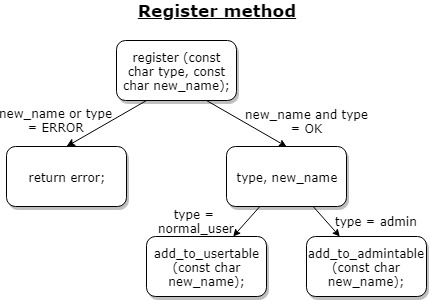
\includegraphics[width=\linewidth]{images/Diagram_register.jpg}
\end{subfigure}%
\begin{subfigure}[H]{.5\linewidth}
    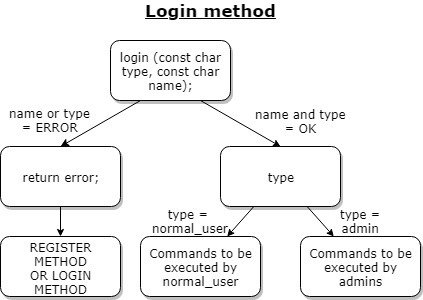
\includegraphics[width=\linewidth]{images/Diagram_login.jpg}
\end{subfigure}
\end{figure}

\endgroup
\vspace*{\fill}

\newpage

\vspace*{\fill}
\begingroup
\centering

\begin{figure}[H]
\centering
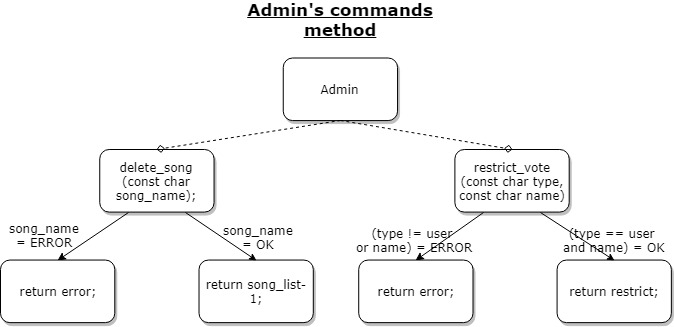
\includegraphics[width=12cm]{images/Diagram_admin_commands.jpg}
\end{figure}

\begin{figure}[H]
\centering
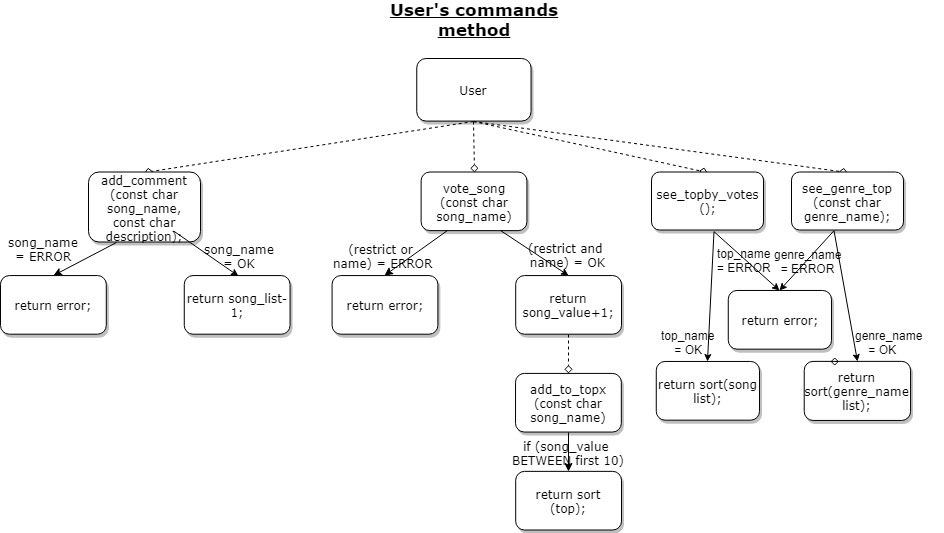
\includegraphics[width=\linewidth]{images/Diagram_user_commands.jpg}
\end{figure}
 
\endgroup
\vspace*{\fill}

\newpage

\vspace*{\fill}
\begingroup
\centering

\begin{figure}[H]
\includegraphics[width=\linewidth]{images/Program_functions.jpg}
\end{figure}
 
\endgroup
\vspace*{\fill}

\newpage

\section{Detalii implementare}

\quad Pentru ca aplicatia sa functioneze in modul dorit, functiile implementate vor trebui sa respecte ultima diagrama. 

Functia de inregistrare are rolul de a inregistra un admin sau un user, in functie de tip si numele dorit, care se va memora in baza de date. Daca tipul este gresit sau numele exista deja in tabela SQL, se va afisa un mesaj de eroare si se va cere o noua inercare sau daca este dorita, iesirea din program. Incercarea poate fi de inregistrare sau logare in cazul in care persoana in cauza are deja un cont. 

Functia de logare functioneaza pe aceleasi principii. Odata logat cu succes, in functie de tip (administrator sau utilizator) se vor putea realiza diverse comenzi. 

Adminul va avea dreptul de a iesi din program, sterge o melodie in functie de numele ei sau de a restrictiona dreptul unui user de a vota. Daca numele melodiei este gresit sau daca numele si tipul utilizatorului nu sunt corecte, se va afisa o eroare. Adminul va putea ulterior rescrie comanda. 

In cadrul functiei de restrictionare, se va seta un parametru special, care, in functie de numele utilizatorului, va restrictiona dreptul de votare al acestuia. 

Utilizatorul poate iesi din program, poate adauga un comentariu la o melodie in functie de numele melodiei, poate sa o voteze si vizualiza topurile. Daca se produce vreo eroare, se va afisa un mesaj iar user-ul va avea dreptul de a rescrie comanda. 

Voturile la melodii vor fi initializate la inceputul prgramului cu 0. Intr-o coloana numita "Restrictionat" din baza de date in dreptul user-ului, prin valoarea 1 se va intelege ca userul are voie sa voteze si prin valoarea -1, ca nu are dreptul de a vota nicio melodie. Legatura intre tabele se va realiza prin Join-uri. Pentru votare, se va verifica intai daca coloana "Restrictionat" are valoare pozitiva (1) si apoi se va actualiza votul pentru melodie prin incrementarea lui cu 1 si vor putea fi actualizate si listele de topuri din cadrul bazei de date. 

Functia de iesire din program va putea fi accesata oricand si va deloga orice client care a cerut acest lucru si are sesiune activa.

Mai jos se afla cateva imagini care prezinta pe scurt cum ar trebui sa functioneze cateva dintre functiile programului:

\begin{lstlisting}[style=CStyle]
//partea de register
if (new_name != (SELECT name FROM users WHERE name = new_name) && strcmp(type, "user") == 0)
	add_to_usertable (new_name);
else if (new_name != (SELECT name FROM admins WHERE name = new_name) && strcmp(type, "admin") == 0)
	add_to_admintable (new_name);
else 
{
	printf (%s, "Incorrect type or name already exists. If you already have an account, try to log in.\n");
}
\end{lstlisting}

\begin{lstlisting}[style=CStyle]
//partea de login
if ( (nume == (SELECT name FROM users WHERE name = nume) && strcmp(type, "user") == 0) 
	//functions to be executed by users
else if (nume == (SELECT name FROM admins WHERE name = nume) &&  strcmp(type, "admin") == 0)
	//functions to be executed by users
else 
{
	printf (%s, "Incorrect type or name already exists.\n");
}
\end{lstlisting}

\begin{lstlisting}[style=CStyle]
//partea de votare (admin)
result = ("SELECT nume FROM users WHERE nume = '%s'", name);
if (type != "user" ||  result != name)
	printf (%s, "Incorect user type or name does not exist!"\n);
else 
	restrict_vote (type, name);

restrict_vote (const char* type, const char* name)
{
	result = ("SELECT nume FROM users WHERE nume = '%s'", name);
	UPDATE users SET restrict = -1 WHERE name = result;
	printf (%s, "Table modified.\n");
} 
\end{lstlisting}

\begin{lstlisting}[style=CStyle]
//partea de votare melodie (user)
result = (SELECT name FROM song WHERE name = song_name);
if (result != song_name)
	printf (%s, "You typed in the wrong name!\n")
else 
{
	if ((SELECT restrict FROM users WHERE name = actual_user) == 1)
		vote_song (song_name);
	else
		printf (%s, "You are restricted from voting any song by an admin!\n")
}

vote_song (const char* song_name)
{
	UPDATE song SET vote = (SELECT vote FROM song WHERE name = song_name)+1 WHERE name = song_name;
}
\end{lstlisting}

\section{Concluzii}

\quad Solutia data ar putea fi imbunatatita prin utilizarea unor chei primare in baza de date, pentru a lega tabelele intre ele. Sintaxele SQL complicate ar fi astfel evitate. In solutia propusa se vor folosi sintaxe pentru join-uri de tabele. De asemenea, o alta imbunatatire ar putea fi efectuata la votare, in asa fel incat un user sa nu poata vota o melodie de mai multe ori si daca exista mai multe melodii cu acelasi numar de voturi ce se pot afla in top, sa existe o departajare a acestora. De asemenea, o varianta mai buna pentru inregistrarea adminilor ar fi ca aceasta sa se poata realiza doar daca un admin este deja inregistrat si logat, pentru a evita riscul ca un user obisnuit sa devina admin.

In privinta tehnologiilor utilizate, un server UDP ar fi mai bun din punctul de vedere al vitezei, fata de TCP. Acesta ar fi mai performant dar nu garanteaza integritatea datelor.

\section{Bibliografie}

Site-uri utilizate:

https://www.youtube.com/watch?v=n5Ed3DA2sbE

https://www.tutorialspoint.com/sqlite/sqliteccpp.htm

https://www.sqlite.org/index.html

http://zetcode.com/db/sqlitec/

https://gist.github.com/jsok/2936764

http://www.wassen.net/sqlite-c.html

https://packages.ubuntu.com/search?keywords=sqlite3

https://linuxhint.com/installsqlitebrowserubuntu1804/

https://askubuntu.com/questions/340603/sqlite-installation

https://www.thoughtco.com/creating-populating-running-database-sql-query-958233

https://stackoverflow.com/questions/28602168/mysql-insert-statement-in-c

https://profs.info.uaic.ro/~computernetworks/

https://sites.google.com/view/fii-rc

https://www.ibm.com/support/knowledgecenter/en/SSLTBW2.1.0/

https://www.cs.dartmouth.edu/~campbell/cs50/socketprogramming.html

https://www.w3schools.com/sql/sqlalter.asp

https://stackoverflow.com/questions/3024546/change-one-cells-data-in-mysql

https://stackoverflow.com/questions/4361774/mysql-update-multiple-tables-with-one-query

http://www.mysqltutorial.org/mysql-update-data.aspx

http://www.mysqltutorial.org/mysql-update-join/

\end{document}